\entry{2026-10-08}{Second-order time stepping (C2, complete)}

Lane \texttt{2026-10-08-jcp-time2} (last commit \texttt{a7a12528f}, mirror \texttt{1445e4735}). Jobs 5012794, 5012974, 5015584, 5017631 (A100), 5020049, 5023437 (H200); all audited, namespace emptied. Every step was Codex-gated, and the final report audit came back clean. Report: \path{worktrees/2026-10-08-jcp-time2/experiments/jcp-time2/report.md}. \textbf{All accuracy numbers are provisional} (first-order references).

\subsection*{2D, accurate setting ($R'=384$, Gauss $96^2$, $1024^2$, 38 cases)}
\begin{itemize}
\item Same step and cost: worst/median error vs ST goes from 2.747/0.906\,\% (backward Euler) to 1.796/0.098\,\% (Crank--Nicolson). Time error falls from 0.978\,\% to 0.026\,\%.
\item At twice the step, Crank--Nicolson gives 1.803/0.259\,\% and runs about 1.75$\times$ faster. Both pre-registered hypotheses pass.
\item Fair comparison: the full solver given the same schemes is also faster and more accurate with Crank--Nicolson. Matched speed-up against it is 1.76$\times$ (backward Euler) and 3.65$\times$ (Crank--Nicolson at $2\Delta t$).
\end{itemize}
\begin{center}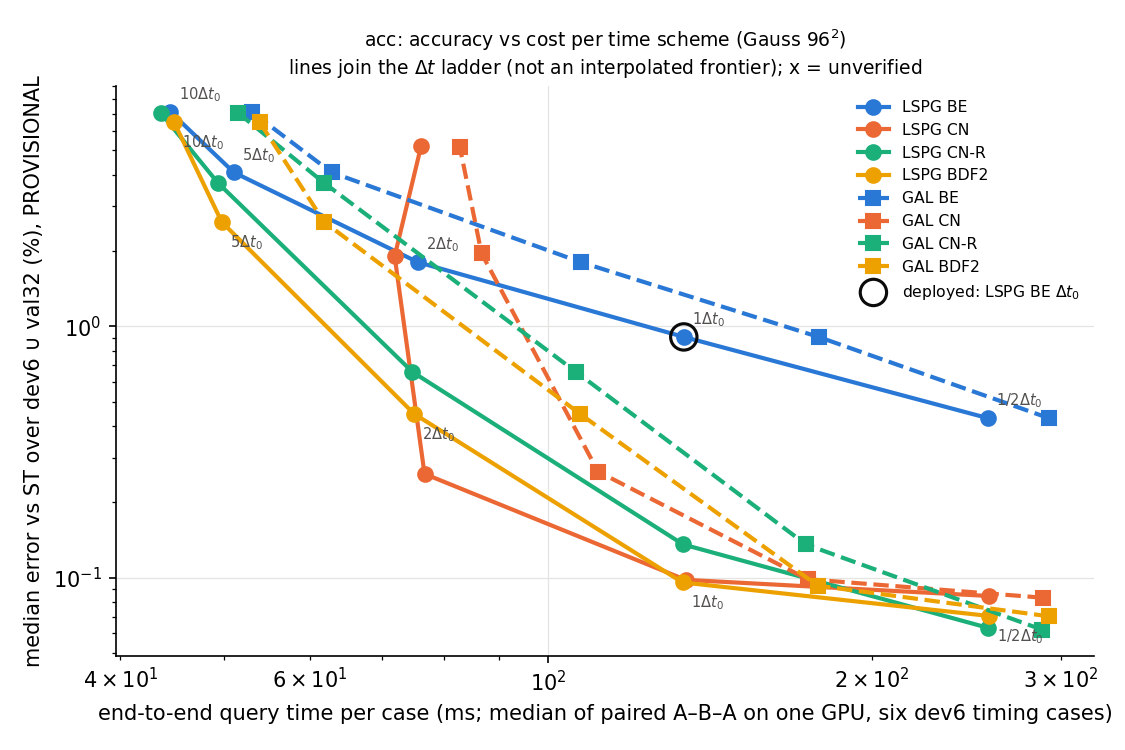
\includegraphics[width=0.8\linewidth]{figs/c2_error_vs_cost_acc.png}\end{center}
\begin{center}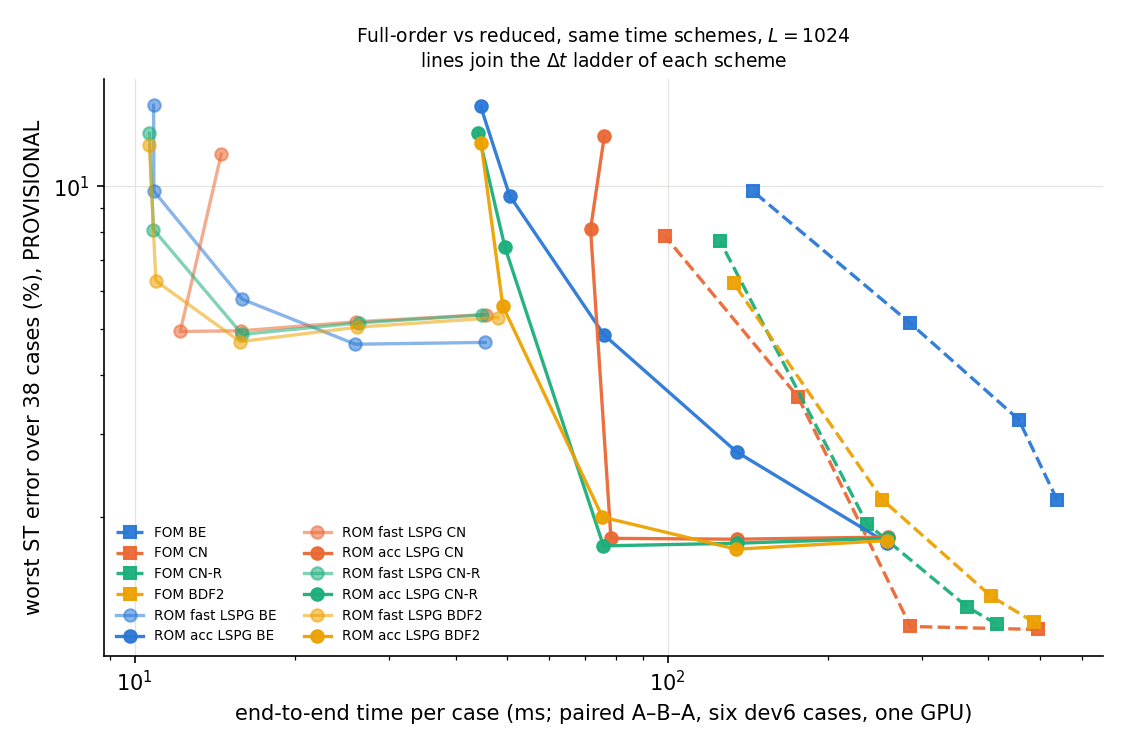
\includegraphics[width=0.8\linewidth]{figs/c2_fom_vs_rom.png}\end{center}

\subsection*{Other settings}
\begin{itemize}
\item Wide ($R'=512$): 2.837/0.907\,\% $\to$ 2.166/0.111\,\%; both hypotheses pass.
\item Fast ($R'=128$): the median improves (1.035 $\to$ 0.419\,\%) but the worst case worsens (4.637 $\to$ 5.171\,\%); both fail, because the small bank's error dominates.
\item 3D ($65^3$, 16 cases): time error drops 21$\times$ (1.87 $\to$ 0.089\,\%) at about equal cost. The generic solver is about 1.7$\times$ the deployed fixed sweep, so the gain is accuracy, not speed. The 3D reference is itself backward Euler at $\Delta t/4$, so it cannot rank the schemes (pre-registered).
\end{itemize}

\subsection*{Retracted or corrected}
\retracted{the ``1--2 percentage points'' of backward-Euler time error is the maximum gap; the median gap is 0.5--0.8 pp. Least-squares Crank--Nicolson is not second order and must not be called so; the Galerkin form and the CN-R/BDF2 least-squares variants are. Comparing against a backward-Euler full solver overstates the speed-up.}

\subsection*{Open}
A fixed-sweep second-order solver for 3D (the route to a 3D speed-up); rerun against second-order references; choose the Galerkin or least-squares form for the paper; test64 and $4096^2$ replication.
